\chapter{Grundlagen}

\section{Software Design}

\subsection{Einführung}

Software-Design ist ein zentraler Aspekt der Softwareentwicklung, der maßgeblich den Erfolg und die Wartbarkeit eines Projekts beeinflusst. Verschiedene architektonische Patterns bieten Lösungen für wiederkehrende Probleme und helfen Entwicklern, robuste und skalierbare Anwendungen zu erstellen. Robert C. Martin, ein Pionier in der Software-Architektur, betont in seinem Buch \textit{Clean Architecture} die Bedeutung von guten Architekturen:

\begin{quote}
The goal of software architecture is to minimize the human resources required to build and maintain the required system. \autocite{martin:clean-architecture}
\end{quote}

Dieses Zitat unterstreicht, dass eine durchdachte Architektur nicht nur die Entwicklungszeit verkürzt, sondern auch die langfristige Wartung vereinfacht. In diesem Kontext werden im Folgenden zwei bedeutende architektonische Patterns vorgestellt, die im Rahmen der Projektdurchführung relevant sind: \ac{ddd} und Microservices.

\subsection{Architektonische Patterns und Ansätze}

\subsubsection{Microservices} \label{cha:grundlagen:swdesign:microservices}

Unter dem Begriff \textit{Microservices} versteht sich der Ansatz, ein Software-System als Orchestration mehrerer Dienste zu unterteilen. Jeder Dienst ist für eine Aufgabe des gesamten System-Kontexts verantwortlich und kann unabhängig von anderen Diensten als ein eigener Prozess laufen. \autocite{LewisFowler2024}

\subsubsection{Domain Driven Design} \label{cha:grundlagen:swdesign:ddd}

Das \textit{\ac{ddd}} ist eine Methodologie, die hauptsächlich bei komplexen Softwareprojekten zum Einsatz kommt. Es gehört weder zur Kategorie der Frameworks noch zu den architektonischen Patterns. Vielmehr ist es eng mit der Denkweise der Microservices, wie in Kapitel \ref{cha:grundlagen:swdesign:microservices} beschrieben, verbunden. Domain-driven Design konzentriert sich darauf, Aktivitäten und Prozesse aus dem realen Leben in die Softwareentwicklung zu abstrahieren. \autocite{LewisFowler2024}

\subsubsection{Onion-Architecture} \label{cha:grundlagen:swdesign:onion}

Die \textit{Onion-Architecture}, auch bekannt als \textit{Clean Architecture}, wurde von Jeffrey Palermo entwickelt und wird insbesondere für C\#-Projekte von Microsoft empfohlen. Sie zielt darauf ab, die typischen Probleme monolithischer Anwendungen, wie hohe Kopplung und geringe Wartbarkeit, zu vermeiden. Die Architektur visualisiert die Software als konzentrische Schichten, vergleichbar mit den Schichten einer Zwiebel. Folgende Abbildung stellt diesen Aufbau nochmals dar:

\begin{figure}[H]
    \centering
    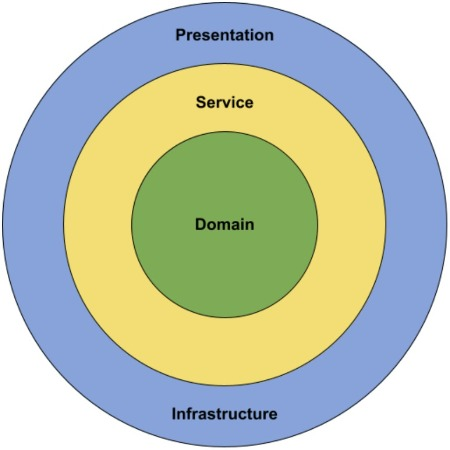
\includegraphics[width=.65\textwidth]{images/PrAR-Grundlagen-OnionArchitecture.jpeg}
    \caption{Bild Onion Architecture, nach \autocite{CodeMaze2024}}
    \label{fig:grundlagen:swdesign:onion}
\end{figure}

\newpage

Die Onion-Architecture gliedert sich in vier Hauptschichten:

\begin{itemize}
\item \textbf{Domain Layer:} Im Zentrum steht die Domäne, die Geschäftslogik und Geschäftsregeln beinhaltet und keinerlei Abhängigkeiten zu äußeren Schichten hat.
\item \textbf{Service Layer:} Diese Schicht enthält die Anwendungsspezifische Logik und nutzt die in der Domain Layer definierten Schnittstellen.
\item \textbf{Infrastructure Layer:} Hier befinden sich Implementierungen für Datenzugriff, Netzwerkkommunikation und andere externe Dienste.
\item \textbf{Presentation Layer:} Diese Schicht ist für die Benutzeroberfläche und die Präsentation der Daten verantwortlich.
\end{itemize}

Konzepte der Onion-Architecture fördern die Abhängigkeit von Abstraktionen (Interfaces) anstatt von konkreten Implementierungen. Diese Abhängigkeitsinversion erlaubt es, Implementierungen zur Laufzeit auszutauschen, was die Flexibilität und Erweiterbarkeit der Software erhöht.

Die Vorteile der Onion-Architecture sind:

\begin{itemize}
\item \textbf{Hohe Testbarkeit:} Da alle Schichten über definierte Schnittstellen kommunizieren, können einzelne Komponenten leicht isoliert und getestet werden.
\item \textbf{Klare Abhängigkeiten:} Abhängigkeiten fließen strikt in Richtung der zentralen Domänenschicht, wodurch höhere Schichten die Implementierungen der unteren Schichten verwenden können, aber nicht umgekehrt.
\item \textbf{Trennung von Geschäftslogik und Implementierungsdetails:} Die Geschäftslogik kann unabhängig von technischen Implementierungsdetails entwickelt werden. Notwendige Schnittstellen zu externen Systemen werden definiert, aber deren konkrete Implementierung wird in den äußeren Schichten gekapselt.
\end{itemize}

Diese Struktur ermöglicht es, komplexe Anwendungen modular zu entwickeln und erleichtert die Wartung und Weiterentwicklung der Software \autocite{CodeMaze2024}.

\subsection{Kollaboration mehrerer Dienste}

\subsubsection{Eventbasierte Architektur: Message Broker und Message Bus} \label{cha:grundlagen:swdesign:kollab:msgbus}

Eine eventbasierte Architektur ermöglicht es, Nachrichten schnell und flexibel zwischen mehreren Diensten auszutauschen. Ein verbreiteter Ansatz hierfür ist die Nutzung eines \textit{Message-Brokers}. Im Folgenden werden die vier grundlegenden Aspekte dieser Architektur beschrieben (vgl. \autocite{oreilly:mod-swarch}):
\begin{enumerate}
    \item \textbf{Initiierendes Event}: Ein \textit{Ereignis}, das den Event-Fluss anstößt und an einen Event-Kanal des Event-Brokers gesendet wird.
    \item \textbf{Event-Broker}: Ein \textit{Orchestrator}, der mehrere Kanäle verwaltet, auf denen Event-Prozessoren lauschen können.
    \item \textbf{Event-Prozessor}: Eine Einheit, die auf einem Kanal lauscht und ein eingehendes Event verarbeitet. Dabei kann ein neues (verarbeitetes) Event erzeugt und an einen anderen Kanal gesendet werden.
    \item \textbf{Das zu verarbeitende Event}: Ein Ereignis, das durch die beschriebenen Mechanismen verarbeitet oder erzeugt wird.
\end{enumerate}

\textbf{Vorteile}

\begin{enumerate}
    \item \textbf{Architektonische Erweiterbarkeit}: Events können vorläufig erzeugt und an den Message-Broker gesendet werden, ohne dass der Event-Prozessor bereits implementiert sein muss. Dies ermöglicht die spätere Implementierung des Prozessors.
    \item \textbf{Abkapselung}: Jedes Modul ist für seine eigene Funktionalität verantwortlich, während alles außerhalb Bestandteil anderer Module ist.
    \item \textbf{Skalierbarkeit}: Events können von mehreren (gleichen) Event-Prozessoren verarbeitet werden. Der Kanal fungiert als FIFO-Warteschlange und ermöglicht eine notwendige Synchronisation.
    \item \textbf{Asynchronität}: Die Kommunikation erfolgt asynchron, was die Entkopplung der Dienste und die Verbesserung der Systemleistung ermöglicht.
\end{enumerate}

\textbf{Nachteile}

\begin{enumerate}
    \item \textbf{(De-)Marshalling}: Nachrichten müssen in ein anderes Format (z.B. JSON, String, Byte-Array) konvertiert und wieder zurückkonvertiert werden. Dies kann die Performance beeinträchtigen.
    \item \textbf{Policies}: In einer traditionellen Message-Broking-Architektur kann theoretisch jeder auf einen Kanal \textit{subscriben}. Es gibt keine klaren Schichten zur Trennung der Zugriffsrechte.
    \item \textbf{Komplexität}: Das Management mehrerer Module und die Nachverfolgung von \textit{Event-Publishern} und \textit{Event-Subscriber} können schwierig sein.
\end{enumerate}

\subsubsection{RESTful APIs} \label{cha:grundlagen:collaboration:rest}

Für die Kommunikation und den Datenaustausch zwischen mehreren Diensten stehen verschiedene Kommunikations-Protokolle zur Verfügung. HTTP ist ein standardisiertes Kommunikationsprotokoll und ist in Bereichen der Web-Anwendungen weit verbreitet.

\ac{rest} definiert kein neues Kommunikationsprotokoll. Es ist ledigliche eine Sammlung von Architekturbeschränkungen und definiert Regeln, die der Entwickler befolgen muss, um eine Zustandslosigkeit in der Kommunikation zu erfüllen \autocite{RedHat2023}.

